% Metódy inžinierskej práce

\documentclass[10pt,twoside,slovak,a4paper]{article}

\usepackage[slovak]{babel}
%\usepackage[T1]{fontenc}
\usepackage[IL2]{fontenc} % lepšia sadzba písmena Ľ než v T1
\usepackage[utf8]{inputenc}
\usepackage{graphicx}
\usepackage{url} % príkaz \url na formátovanie URL
\usepackage{hyperref} % odkazy v texte budú aktívne (pri niektorých triedach dokumentov spôsobuje posun textu)

\usepackage{cite}
%\usepackage{times}

\pagestyle{headings}

\title{Metódy strojového učenia a ich praktické použitie\thanks{Semestrálny projekt v predmete Metódy inžinierskej práce, ak. rok 2021/22, vedenie: Ing. Fedor Lehocki}} 

\author{Martin Orlej\\[2pt]
	{\small Slovenská technická univerzita v Bratislave}\\
	{\small Fakulta informatiky a informačných technológií}\\
	}

\date{\small 11. oktober 2021} 



\begin{document}

\maketitle

\begin{abstract}
Strojové učenie sa v posledných rokoch čoraz viac spomína či už vo vedeckých prácach, alebo v rôznych článkoch, zameraných na technológie. Či už ide o niečo jednoduché, ako aplikácie na telefóny, alebo o vysoko pokročilé technológie ako autonómne jazdenie a počítačové videnie. V mojej práci by som sa chcel zamerať na rôzne modely strojového učenia, ako napr. lineárna regresia, Boltzmannove stroje alebo transformátory, na ich praktické a najefektívnejšie využitie, napríklad pri spracovávaní veľkého množstva údajov, spracovávaní jazyka (NLP) alebo počítačovom videní a klasifikácii, a na slabé miesta a nevýhody týchto modelov. Rád by som taktiež jednoducho opísal aj už existujúci systém, ako algoritmus GPT-3 vyvinutý nadáciou OpenAI, a možnosti jeho využitia.
\end{abstract}









\section{Nejaká časť} \label{nejaka}

Z obr.~\ref{f:rozhod} je všetko jasné. 

\begin{figure*}[tbh]
\centering
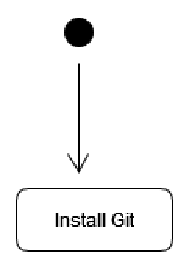
\includegraphics[scale=1.0]{diagram.pdf}
\caption{Diagram 1}
\paragraph{Poznámka} Aj text môže byť prezentovaný ako obrázok. Stane sa z neho označný plávajúci objekt. Po vytvorení diagramu zrušte znak \texttt{\%} pred príkazom \verb|\includegraphics| označte tento riadok ako komentár (tiež pomocou znaku \texttt{\%}).

\label{f:rozhod}
\end{figure*}

\hfil
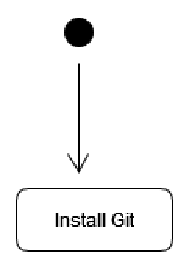
\includegraphics[scale=1.0, angle=90]{diagram.pdf}
\hfil
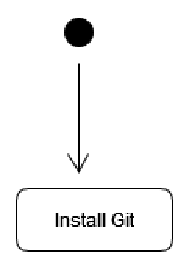
\includegraphics[scale=1.0]{diagram.pdf}
\hfil

\paragraph{Úvod} V tejto časti je popísaný úvod k práci s krátkym popisom

\section{Tabuľka} \label{časť textu}

\begin{tabular}{lc}
Metódy inžinierskej práce & 2000 \\
Procedurálne programovanie & 3000 \\
Matematická analýza & 4000 \\
Anglický jazyk & 7000 \\
\end{tabular}

\section{Iná časť} \label{ina}

Základným problémom je teda\ldots{} Najprv sa pozrieme na nejaké vysvetlenie (časť~\ref{ina:nejake}), a potom na ešte nejaké (časť~\ref{ina:nejake}).

Môže sa zdať, že problém vlastne nejestvuje\cite{Coplien:MPD}, ale bolo dokázané, že to tak nie je~\cite{Czarnecki:Staged, Czarnecki:Progress}. Napriek tomu, aj dnes na webe narazíme na všelijaké pochybné názory\cite{PLP-Framework}. Dôležité veci možno \emph{zdôrazniť kurzívou}.


\subsection{Nejaké vysvetlenie} \label{ina:nejake}


\subsection{Ešte nejaké vysvetlenie} \label{ina:este}

\paragraph{Veľmi dôležitá poznámka.}
Niekedy je potrebné nadpisom označiť odsek. Text pokračuje hneď za nadpisom.



\section{Dôležitá časť} \label{dolezita}




\section{Ešte dôležitejšia časť} \label{dolezitejsia}




\section{Záver} \label{zaver} % prípadne iný variant názvu



%\acknowledgement{Ak niekomu chcete poďakovať\ldots}


% týmto sa generuje zoznam literatúry z obsahu súboru literatura.bib podľa toho, na čo sa v článku odkazujete
\bibliography{literatura}
\bibliographystyle{plain} % prípadne alpha, abbrv alebo hociktorý iný
\end{document}
